\setcounter{chapCompteur}{3}
\ChapNumber{\myChapNum}{\hspace*{0.8cm}\LARGE \textbf{En terminal}}{\hspace*{0.8cm}\small Du classeur à la grille}
\section{S'en servir en ligne de commande}

\begin{frame}[t,fragile]{Deux façons d'utiliser Dim2Dir : un fichier ou pip}
% [DEVELOPPE: commandes d'installation]
\vfill
{\relscale{0.9}
Python 3.10 ou plus ; même code, même API. Classeur : en-têtes contigus en ligne 1, essais dès la ligne 2.
\par\vspace{0.3em}\noindent\textbf{Fichier seul : installer d'abord ses dépendances}
\begin{lstlisting}[style=py_style1,language={},numbers=none,basicstyle=\ttfamily\footnotesize,xleftmargin=0pt,breakatwhitespace=false,breakindent=0pt,keepspaces=true,breaklines=true]
python -m pip install "openpyxl>=3.1" "matplotlib>=3.7" "pillow>=10"
\end{lstlisting}
\begin{columns}[T,totalwidth=1.05\textwidth]
\begin{column}{0.49\textwidth}
\textbf{Télécharger \texttt{Dim2Dir.py}}
\begin{lstlisting}[style=py_style1,language={},numbers=none,basicstyle=\ttfamily\footnotesize,xleftmargin=0pt,breakatwhitespace=false,breakindent=0pt,keepspaces=true,breaklines=true]
python Dim2Dir.py plan.xlsx
\end{lstlisting}
\end{column}
\begin{column}{0.49\textwidth}
\textbf{Installer le paquet}
\begin{lstlisting}[style=py_style1,language={},numbers=none,basicstyle=\ttfamily\footnotesize,xleftmargin=0pt,breakatwhitespace=false,breakindent=0pt,keepspaces=true,breaklines=true]
pip install dim2dir
dim2dir plan.xlsx Feuil1 --output-dir resultats
\end{lstlisting}
Feuille par défaut de la ligne de commande : \texttt{Feuil1} si elle existe, sinon la première. L'API prend la première.
\end{column}
\end{columns}
Extras : \texttt{[pandas]} ajoute les DataFrames (tableaux pandas), \texttt{[excel]} exige Windows et Excel.}
\note{Autres appels : python -m dim2dir plan.xlsx ; pip install dim2dir[pandas] ; pip install dim2dir[excel]. Sans argument, la ligne de commande lit ./Dim2Dir.xlsx, feuille Feuil1 si elle existe, sinon la première. Le fichier autonome peut aussi être importé depuis un programme placé à côté. Sous Windows, Lancer_Dim2Dir.bat accepte un classeur glissé dessus. Le lanceur est livré dans le dépôt. L'installation pip n'installe pas ce lanceur.}
\vfill
\end{frame}

\begin{frame}[t]{Les options choisissent les sorties et personnalisent le rendu}
% [DEVELOPPE: tableaux d'options]
\vfill
{\footnotesize\setlength{\tabcolsep}{3pt}
\begin{columns}[T,totalwidth=1.05\textwidth]
\begin{column}{0.49\textwidth}
\begin{tabular}{@{}>{\raggedright\arraybackslash}p{0.54\linewidth}>{\raggedright\arraybackslash}p{0.42\linewidth}@{}}
\toprule
\textbf{Sélection et sorties} & \textbf{Effet}\\
\midrule
\texttt{excel\_file}, \texttt{sheet\_name} & Source et feuille\\
\texttt{-{}-all-sheets}, \texttt{-{}-list-sheets} & Traiter tout, lister\\
\texttt{-{}-output-dir} & Dossier de sortie\\
\texttt{-{}-outputs xlsx,png,pdf,svg} & Formats demandés\\
\texttt{-{}-image-engine}, \texttt{-{}-dpi} & Moteur, dpi (points par pouce)\\
\texttt{-{}-x-factors}, \texttt{-{}-y-factors} & Partition des facteurs\\
\texttt{-{}-report}, \texttt{-{}-dry-run} & JSON, sans écriture\\
\texttt{-{}-max-cells}, \texttt{-{}-max-pixels} & Plafonds grille, image\\
\texttt{-{}-max-runs}, \texttt{-{}-excel-timeout} & Essais, délai Excel\\
\bottomrule
\end{tabular}
\end{column}
\begin{column}{0.49\textwidth}
\begin{tabular}{@{}>{\raggedright\arraybackslash}p{0.54\linewidth}>{\raggedright\arraybackslash}p{0.42\linewidth}@{}}
\toprule
\textbf{Personnalisation} & \textbf{Effet}\\
\midrule
\texttt{-{}-style fichier.json} & Charger un Style\\
\texttt{-{}-palette}, \texttt{-{}-palette-reverse} & Palette (gamme de couleurs), inversion\\
\texttt{-{}-color}, \texttt{-{}-font-color} & Base, texte\\
\texttt{-{}-font}, \texttt{-{}-font-size} & Police, points\\
\texttt{-{}-cell-size}, \texttt{-{}-label-scale} & Cellule, étiquettes\\
\texttt{-{}-line-color}, \texttt{-{}-line-style} & Bordures\\
\texttt{-{}-title}, \texttt{-{}-no-title} & Titre, suppression\\
\texttt{-{}-legend}, \texttt{-{}-label-format} & Légende, format y\\
\texttt{-{}-run-prefix}, \texttt{-{}-level-order} & Préfixe, niveaux\\
\bottomrule
\end{tabular}
\end{column}
\end{columns}
\vspace{0.5em}
Les options explicites priment sur le JSON. \texttt{-{}-outputs} remplace \texttt{-{}-no-xlsx}, \texttt{-{}-no-png} et \texttt{-{}-no-pdf}. L'aide \texttt{-{}-help} détaille les valeurs acceptées.
}
\note{Défauts : source ./Dim2Dir.xlsx, feuille Feuil1, dossier de la source, moteur matplotlib, dpi 200 (50 à 600). Formats par défaut : xlsx,png,pdf. Limites : 90000 cellules, 60000000 pixels, 20000 essais, 120 secondes. --quiet masque résumé et avertissements, --version affiche la version. --level-order est répétable. --font-size : 4 à 72 ; --cell-size : 12 à 120 ; --label-scale : 0.5 à 3. --color accepte RRGGBB sans dièse. --line-style : none, thin, medium, thick. Aucun équivalent CLI de cell_font_color : utiliser le JSON.}
\vfill
\end{frame}

\begin{frame}[t]{Les trois sorties usuelles se complètent d'un SVG}
\vfill
\begin{columns}[T,totalwidth=1.05\textwidth]
\begin{column}{0.54\textwidth}
\centering
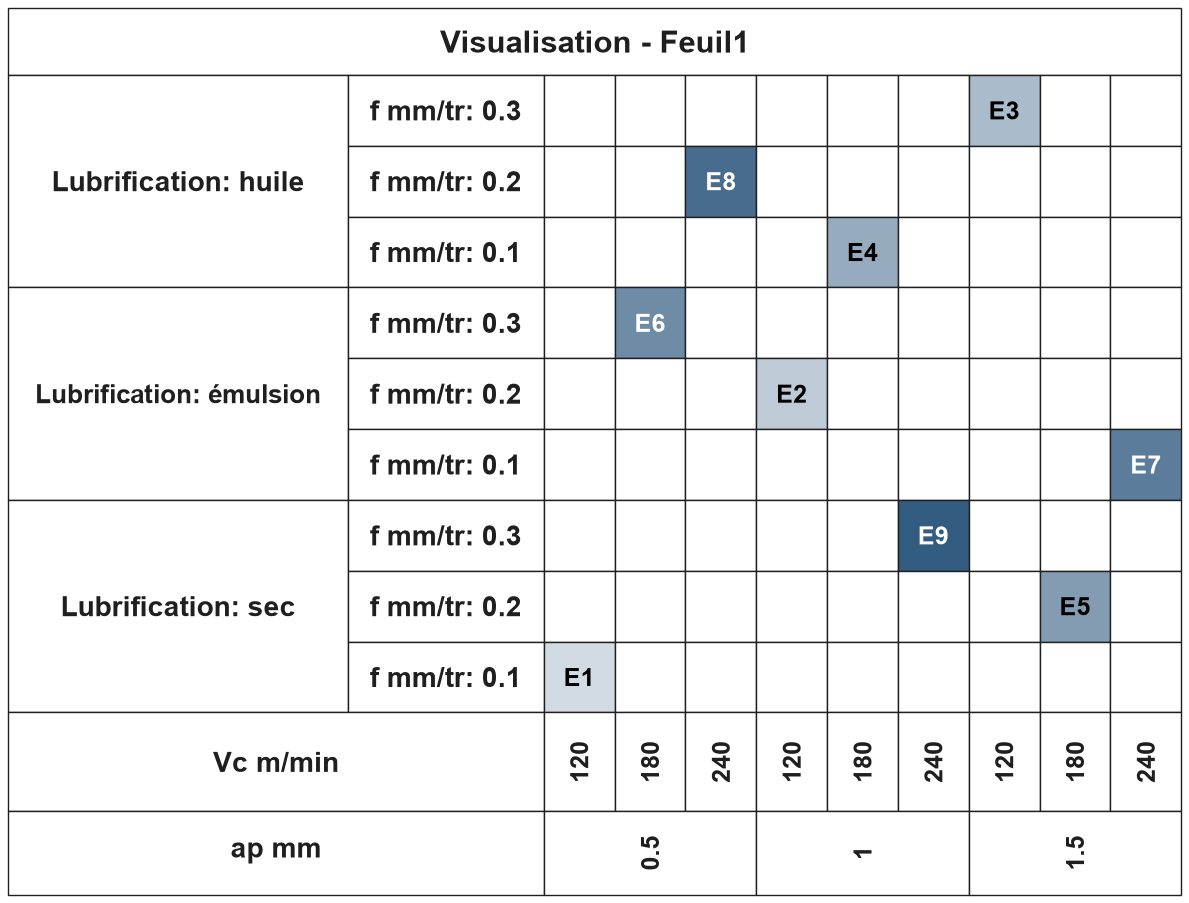
\includegraphics[width=\linewidth,height=0.5\textheight,keepaspectratio]{./_FIG/FIG_Partie_00/tournage_L9.png}
\end{column}
\begin{column}{0.44\textwidth}
\raggedright
{\relscale{0.9}
\begin{tabular}{@{}ll@{}}
\toprule
XLSX & Tableau et dessin\\
PDF & Figure vectorielle\\
PNG & Image selon les dpi\\
SVG & Vectoriel, sur demande\\
\bottomrule
\end{tabular}

\vspace{0.4em}
Neuf cases occupées sur 81 possibles : couverture de 11,1\,\%.
\begin{mybox3}[orange!5!white][Framaorange][Framaorange]{\textbf{Intégrité du classeur}}\footnotesize
La source reste intacte. Dans la copie, openpyxl peut perdre images, graphiques et formes. La zone à droite du tableau doit être libre.
\end{mybox3}}
\end{column}
\end{columns}
{\footnotesize Pour \texttt{plan.xlsx}, feuille \texttt{Feuil1} : \texttt{plan\_visu.xlsx}, \texttt{plan\_visu\_Feuil1.png} et \texttt{.pdf} (SVG sur demande). Exemple pandas : \texttt{resultats\_pandas/plan\_visu\_Feuil1.png}. Figure : \texttt{tournage\_L9.xlsx}, données synthétiques.}
\note{Le SVG exige le moteur matplotlib. Les PDF, PNG et SVG montrent uniquement la zone de visualisation. Les trois sorties usuelles correspondent aux formats par défaut pour une source xlsx. E1 : 120 m/min, 0,1 mm/tr, ap 0,5 mm, à sec.}
\vfill
\end{frame}

\begin{frame}[t,fragile]{Changer les axes réorganise le même factoriel de soudage}
\vfill
{\relscale{0.9}
Le plan $2^4$ (factoriel complet : quatre facteurs à deux niveaux) compte seize essais synthétiques, qui occupent toute la grille $4\times4$. L'affectation des axes change les voisinages, pas les combinaisons.
\begin{columns}[T,totalwidth=1.05\textwidth]
\begin{column}{0.49\textwidth}
\centering\textbf{Défaut : x = I, Gaz}\\[0.3em]
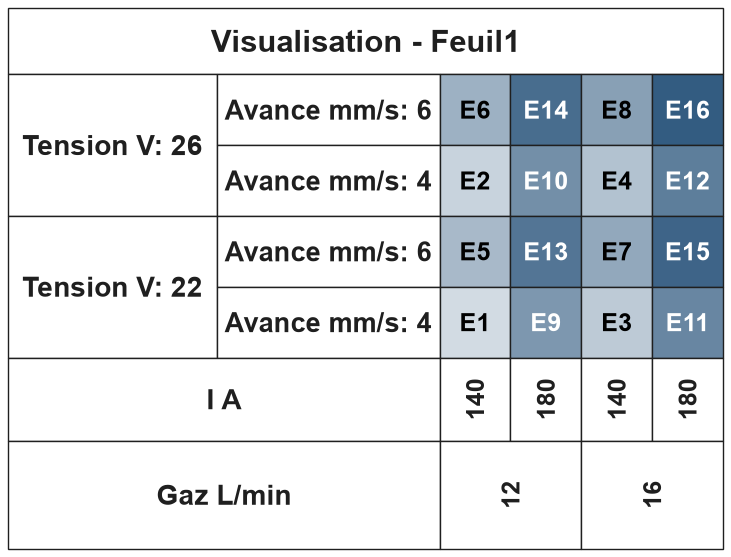
\includegraphics[width=\linewidth,height=0.36\textheight,keepaspectratio]{./_FIG/FIG_Partie_00/soudage_2p4.png}
\end{column}
\begin{column}{0.49\textwidth}
\centering\textbf{Variante : x = I, Avance}\\[0.3em]
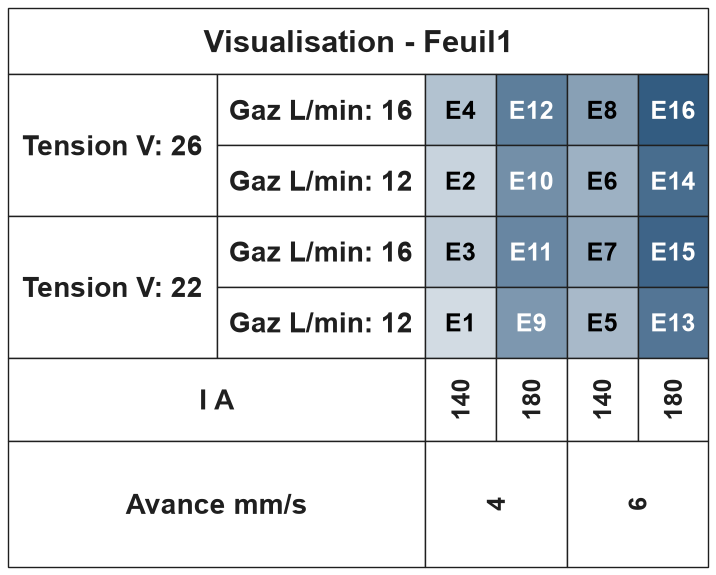
\includegraphics[width=\linewidth,height=0.36\textheight,keepaspectratio]{./_FIG/FIG_Partie_00/soudage_axes_alt.png}
\end{column}
\end{columns}
\vspace{0.4em}
{\footnotesize\ttfamily
-{}-x-factors "I A,Avance mm/s"\\
-{}-y-factors "Gaz L/min,Tension V"}
\notelibre[\footnotesize]{Sorties du même \texttt{soudage\_2p4.xlsx}. À gauche, y porte Avance et Tension. À droite, y porte Gaz et Tension.}}
\note{Les deux listes doivent partitionner exactement les facteurs, hors Run. Leur premier facteur varie le plus vite.}
\vfill
\end{frame}

\begin{frame}[t]{Ce qu'il faut retenir}{Dépannage et bonnes pratiques}
\vfill
{\relscale{0.9}
\begin{mybox3}[yellow!8!white][Framajaune][Framajaune]{\textbf{Points clés}}
\begin{itemize}\itemsep4pt
\item Sortie ouverte dans Excel : la fermer avant de relancer.
\item Feuille introuvable : le message liste les feuilles.
\item Formule sans cache : recalculer et enregistrer le classeur dans Excel.
\item Lire le résumé et les avertissements avant d'interpréter la grille.
\item Essayer d'abord avec \texttt{-{}-dry-run}, qui n'écrit aucun fichier.
\end{itemize}
\end{mybox3}
La simulation vérifie le tableau et sa couverture. Contrôler ensuite la grille exportée, surtout après un changement d'axes ou de limites.}
\note{Le programme ne recalcule pas les formules : il lit leur valeur en cache. Le rapport JSON conserve les avertissements d'un traitement, sauf en simulation qui n'écrit rien.}
\vfill
\end{frame}

\begin{frame}[plain]
\centering\vspace{1cm}
\textbf{\Huge Intégrer la visualisation}
\vspace{1cm}

{\large Et dans votre propre programme Python~?}
\end{frame}
